\subsection{Time-series Dense Encoder}
\textbf{TiDE} (Time-series Dense Encoder) là một mô hình dự báo chuỗi thời gian. Mô hình hoạt động mã hóa chuỗi thời gian quá khứ cùng với hiệp phương sai bằng cách sử dụng “dense MLP” (Multi-Layer Perceptron). Sau đó, mô hình giải mã (decode) chuỗi thời gian được mã hóa (encode) cùng với các hiệp phương sai trong tương lai.

Kiến trúc tổng quan được trình bày ở Hình 1. Đầu vào (input) của mô hình là dữ liệu quá khứ và phương sai của một chuỗi thời gian tại một thời điểm ($y_{1:L}^{(i)}, x_{1:L}^{(i)}, a^{(i)}$) và ánh xạ tới dự đoán của chuỗi thời gian $\hat{y}_{L+1:L+H}^{(i)}$. Thành phần chính của mô hình là residual block MLP.

\textbf{Residual Block:} Là một thành phần quan trọng của kiến trúc TiDE vì nó cho phép mô hình nắm bắt các tính chất phi tuyến tính vốn có trong dữ liệu chuỗi thời gian, đồng thời duy trì các mối quan hệ tuyến tính nhằm giúp cải thiện hiệu suất dự báo dài hạn. 

Mô hình được chia thành hai phần: mã hóa (encoding) và giải mã (decoding):

\textbf{Mã hóa (Encoding):} Nhiệm vụ của bước mã hóa là ánh xạ dữ liệu quá khứ và phương sai của chuỗi thời gian thành một biểu diễn dày đặc (dense). Quá trình mã hóa có hai bước chính

Feature Projection: Sử dụng residual block để ánh xạ $x_t^{(i)}$ tại mỗi time-step, hoạt động này được mô tả như sau
\begin{equation}
    \tilde{x}_t^{(i)} = \text{ResidualBlock}(x_t^{(i)}) 
\end{equation}

\begin{figure}[h]
    \centering
    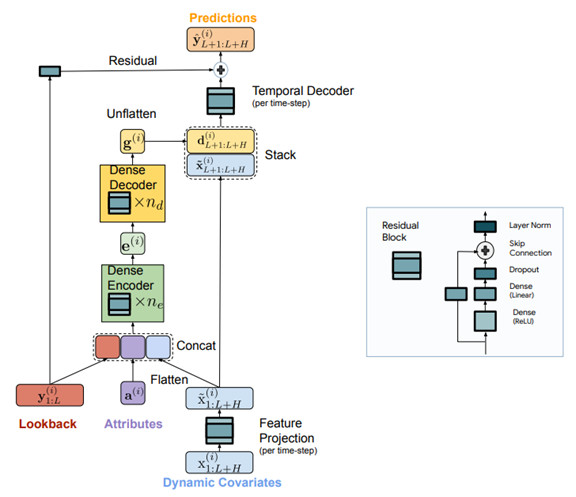
\includegraphics[width=0.5\textwidth]{img/TiDE.png}
    \caption{Tổng quan về kiến trúc TiDE}
    \label{fig:your_figure_label}
\end{figure}

\textbf{Giải mã (Decoding):} Việc giải mã trong mô hình ánh xạ các biểu diễn ẩn được mã hóa thành các dự đoán trong tương lai của chuỗi thời gian. Nó cũng bao gồm hai hoạt động, bộ giải mã dày đặc (dense decoder) và bộ giải mã tạm thời (temporal decoder).

